\documentclass[a4paper,twoside]{report}
%Rahmendatei f�r das Cover

\usepackage{graphicx}
\usepackage{dsfont}

\usepackage{epsf,amsthm,amsmath}
\usepackage[ngerman]{babel}
\usepackage[latin1]{inputenc}
\usepackage{graphicx}
\setlength{\parskip}{5pt plus 8pt minus 2pt}
\pagestyle{headings}

%----------------------------------------------------------------------
%  Makros
%----------------------------------------------------------------------
%\usepackage{dsfont}
%\def\C{\mathds{C}}
%\def\F{\mathds{F}}
%\def\R{\mathds{R}}
%\def\N{\mathds{N}}
%\def\Z{\mathds{Z}}
%
%\newcommand{\bra}[1]{\langle#1|}
%\newcommand{\ket}[1]{|#1\rangle}
%\newcommand{\braket}[2]{\langle#1|#2\rangle}
%\newcommand{\ketbra}[2]{|#1\rangle\langle#2|}
%\newcommand{\projektor}[1]{|#1\rangle\langle#1|}
%\newcommand{\schnitt}[2]{
%   \raise3pt\vbox{\moveright6.5pt\hbox{$#1$}}\hspace*{-4pt}\Bigm/
%   \lower3pt\vbox{\moveleft6.5pt\hbox{$#2$}}}
%
%\newcommand{\includeeps}[2]{
%   \def\epsfsize##1##2{#2##1}
%   \centerline{\epsffile{#1}}}
%
%\newtheorem{satz}{Satz}[chapter]
%\newtheorem{bem}[satz]{Bemerkung}
%\newtheorem{lem}[satz]{Lemma}
%\newtheorem{defi}[satz]{Definition}
%\newtheorem{beispiel}[satz]{Beispiel}
%----------------------------------------------------------------------

\begin{document}
\begin{titlepage}
\ \vfill
\Large
\begin{center}
{\LARGE\bf Proseminar} \\[1cm]
{\huge\bf K"unstliche Intelligenz\par}
\vspace*{1cm}
\input unilogo
\unilogo{30}\\[1cm]
{\bf Universit"at Karlsruhe (TH)}\\
{Fakult"at f"ur Informatik}\\
{\em Institut f"ur Algorithmen und Kognitive Systeme}
\vfill
Prof.~Dr.~J.~Calmet\\
Dipl.-Inform.~A.~Daemi
\vfill\vfill 
Wintersemester 2003/2004
\vfill
\vfill
\end{center}
\end{titlepage} 
% 
%\newpage
%\thispagestyle{empty}
%\ 
%\newpage 
\thispagestyle{empty}
\ 
\vfill
\noindent
Copyright $\copyright$ 2003\\
Institut f"ur Algorithmen und Kognitive Systeme\\
Fakult"at f"ur Informatik\\
Universit"at Karlsruhe\\
Am Fasanengarten 5\\
76\,128 Karlsruhe

%\newpage 
%\thispagestyle{empty}
%\ 
%\newpage 



\title{Allgemeine und Heuristische Suchverfahren}
\author{Henning Eberhardt \\ Clemens Lode}

%Rahmendatei f�r Titel, Autor und Inhaltsverzeichniss
\date{}
\maketitle

%\thispagestyle{empty}
%\newpage 

\pagenumbering{roman}
\tableofcontents

%\newpage 
\pagenumbering{arabic}


\setcounter{chapter}{0}
\chapter{Allgemeine und Heuristische Suchverfahren}

%---------------------------------------------------------
%Hier beginnt das eigentliche Dokument 
%---------------------------------------------------------
%Die Ausarbeitung sollte immer eine Einf�hrung in die behandelnden Themen enthalten
\section{Einleitung}

Das Suchen einer L"oesung ist der zentrale Bestandteil der Informatik, ja vielleicht sogar des ganzen Lebens. Von der t"aglichen Suche nach den Schl"usseln mit Hilfe von Erinnerungsstrategien (,,Wo habe ich sie zuletzt gesehen?``) bis zur Suche nach auserirdischer Intelligenz im Weltraum, immer steht man vor endlos vielen M"oglichkeiten.
Diese Ausarbeitung wird sich darauf beschr"anken, Graphenprobleme zu analysieren und verschiedene Algorithmen vorzustellen, die diese effizient l"osen k"onnen.

Grundlage werden die \emph{allgemeinen} oder auch \emph{informierten Suchverfahren} spielen, die eine L"osung schrittweise zusammensetzen, indem sie den Graphen geschickt durchschreitet und jeweils pr"uft ob dieser Schritt Teil der L"osung oder die L"osung selbst ist.

Anschliessend werden Algorithmen erl"autert, die durch Hinzunahme zus"atzlicher Informationen von au"sen die durchschnittliche Suchdauer reduzieren. Eine Gruppe der sogenannten \emph{heuristischen Suchverfahren} baut wie die allgemeinen Suchverfahren die L"osung schrittweise auf, w"ahrend die andere fertige L"osungen erstellt und diese schrittweise optimiert.
Es wird auch ein Ausblick auf moderne Suchalgorithmen, den sogenannten \emph{Genetischen Algorithmen} gegeben, die zunehmend Anwendung in der Wirtschaft wie auch in der Wissenschaft finden.

Zus"atzlich zu den Beispielen der Pfadsuche durch Graphen werden die Algorithmen anhand von sogenannter \emph{Constraint Satisfaction Problems} erkl"art und zum Teil auf deren Schw"achen und St"arken eingegangen.

\section{Allgemeine Suchverfahren}


\section{Allgemeine Suchverfahren}

%Problem consists of four parts:
%Initial state:

%A set of actions:

%A goal test function:

%Path cost function:

%The enviroment of the problem is represented by a state space which we search.

Ein universeller TREESEARCH Algorithmus kann zur Loesung jedes beliebigen Problems eingesetzt werden, es gibt jedoch verschiedene Suchstrategien mit unterschiedlichen Vor und Nachteilen. Die unterschiedlichen Algorithmen werden nach den Kriterien

\begin{itemize}
\item Vollstaendigkeit (completness)
\item Optimalitaet (optimality)
\item Zeitkomplexitaet (time complexity)
\item Speicherbedarf (space complexity)
\end{itemize}

\begin{samepage}
\textbf{\texttt{\begin{tabbing}\quad\quad\=\quad\quad\=\quad\quad\kill
TREESEARCH:\\
function TREESEARCH(problem, fringe) returns a solution, or failure\\
\>fringe <- INSERT( MAKE-NODE( INITIAL-STATE[problem], fringe))\\
\>loop do\\
\>\>if EMPTY?(fringe) then return failure\\
\>\>node <- REMOVE-FIRST(fringe)\\
\>\>if GOAL-TEST[problem] applied to STATE[node] succeeds\\
\>\>then return SOLUTION(node)\\
%Tab rausgenommen, da kommt Latexfehler... nochmal nachlesen
\>fringe <- INSERT-ALL( EXPAND(node, problem), fringe)\\
\\
function EXPAND(node, problem) returns a set of nodes\\
\>successors <- the empty set\\
\>for each <action, result> in SUCCESSOR-FN[problem](STATE[node]) do\\
\>\>s <- a new NODE\\
\>\>STATE[s] <- result\\
\>\>PARENT-NODE[s] <- node\\
\>\>ACTION[s] <- action\\
\>\>PATH-COST[s] <- PATH-COST[node] + STEP-COST(node, action, s)\\
\>\>DEPTH[s] <- DEPTH[node] +1\\
\>\>Add s to successors\\
\>Return sucessors
\end{tabbing}}}
\end{samepage}


Die Komplexitaet haengt vom Verzweigungsfaktor b(branchingfactor) des durchsuchten Zustandsraumes und der Tiefe d(depth) des Suchbaumes ab.
Der Verzweigungsfaktor gibt die Anzahl der Verzweigungen pro Knoten an. Mit seiner Hilfe und der Tiefe d laesst sich also leicht eine Obergrenze fuer die maximale Anzahl  der Knoten in einem Suchbaum angeben:

1 + b + b^{2} + b^{3} + b^{4} .... + b^{d} =  \sum {i=0}^{n}\qquad b^{i}

\subsection{Breitensuche (breadth-first search):}

Bei der Breitensuche, welche von Moore 1959 zur Loesung von Labyrinthen entwickelt wurde, werden jeweils alle Knoten mit der selben Tiefe durchsucht. Der Suchbaum wird also Ebenenweise durchsucht. Dies laesst sich durch den Aufruf TREE-SEARCH(problem, FIFO-QUEUE()) (first in , first out) bewerkstelliegen).

<Picture p74>
\begin{itemize}
\item Vollstaendig: Ja, sofern ein Ziel in einer endlichen Tiefe existiert und der Verzweigungsfaktor endlich ist
\item Optimal: Ja, sofern alle Pfadkosten identisch sind
\item Zeit/Speicheraufwand: O(b^{d+1})
\end{itemize} 


Beispiel:
Geg.: Suchbaum mit Knotengroesse 1kbyte und 10 Verzweigungen pro Knoten(b=10) sowie einem Rechner, der 10.000 Knoten pro Sekunde bearbeitet.

%todo Tabelle
\begin{tabular}{|l|l|l|l|}
\hline
Tiefe & Knoten & Dauer & Speicherverbrauch\\
\hline
2 & 1100 & 0.11 s & 1 Mb\\
\hline
4 & 111100 & 11 s & 106 Mb\\
\hline
6 & \(10^{7}\) & 19 m & 10 Gb\\
\hline
8 & \(10^{9}\) & 31 h & 1 Tb\\
\hline
10 & \(10^{11}\) & 129 d & 101 Tb\\
\hline
12 & \(10^{13}\) & 35 y & 10 P(eta)b\\
\hline
14 & \(10^{15}\) & 3523 y & 1 E(xa)b\\
\hline
\end{tabular}
\textit{ Beispiel aus Artificial Intelligence A modern Approach von Stuart Russel und Peter Norvig Seite 74} 


\subsection{Uniform-cost Search}

Bei dieser Art der Suche, welche auf dem kuerzesten weg zwischen 2 Punkten Algorithmus von Dijkstra  aus dem Jahre 1959 beruht, wird immer der Knoten mit den niedrigsten Pfadkosten gewaehlt, unterscheiden sich die Pfadkosten also nicht liegt eine normale Breitensuche vor. Wenn dieser Algorithmus auf eine Schleife mit den Pfadkosten 0 stoesst, bleibt er dort stecken. Daraus resultiert folgendes:

\begin{itemize}
\item Vollstaendigkeit und Optimalitaet: Sofern alle Pfadkosten >= e > 0
\item Zeit-/Speicheraufwand: O( b^{top(C*/e)}) wobei C* den kosten fuer die Optimale Loesung entspricht -> Es werden viele kleine Schritte bevorzugt, auch wenn diese nicht zum gewuenschten Ziel fuehren.
\end{itemize} 


\subsection{Tiefensuche (Depth-first search)}

Bei der Tiefensuche wird zunaechst der tiefste Knoten im aktuellen Teilstueck des Suchbaumes gewaehlt. Sollte ein Knoten keine (noch nicht durchsuchten) Kinder haben, so sprint der Algorithmus zum Vater dieses Knoten zurueck. Alle durchsuchten Knoten, die nicht zwischen Wurzel und aktuellem Knoten liegen, werden fallengelassen. Tiefensuche entspricht also dem Aufruf TREE-SEARCH(problem, LIFO-QUEUE()) (last in, first out).

Picture p76
\begin{itemize}
\item Vollstaendig: Nur, wenn der Suchbaum ausschliesslich Aeste endlicher Laenge  enthaelt.
\item Optimal: Nein
\item Zeitaufwand: O( b^{d+1})
\item Speicheraufwand: O( b*m ) im Sonderfall backtracking search: O(m)
\textit{(m sei die maximale Suchtiefe)}
\end{itemize}


\subsection{Begrenzte Tiefensuche (Depth-limited search)}

Depthlimited search ist eine Tiefensuche mit eine maximalen Suchtiefe l. Alle Knoten der Tiefe l werden behandelt, als besaessen sie keine Kinder. Tiefensuche entspricht damit DLS mit l = unendlich.

\begin{itemize}
\item Vollstaendig: Nur wenn gilt l >= m
\item Optimal: Nur wenn gilt l=d
\item Zeitaufwand: O(b^{l})
\item Speicheraufwand: O(bl)
\end{itemize}

\begin{samepage}
\textbf{\texttt{\begin{tabbing}\quad\quad\=\quad\quad\=\quad\quad\kill
Function DEPTH-LIMITED-SEARCH(problem, limit) returns a solution, or failure/cutoff\\
\>Return RECURSIVE-DLS( MAKE-NODE( INITIAL-STATE[problem]), problem, limit)\\
\\
Function RECURSIVE-DLS(node, problem, limit) returns a solution or failure/cutoff\\
\>Cutoff\_occurred? <- false\\
\>If GOAL-TEST[problem](STATE[node]) then return SOLUTION(node)\\
\>Else if DEPTH[node] = limit then return cutoff\\
\>Else for each successor in EXPAND(node, problem) do\\
\>\>Result <- RECURSIVE-DLS(successor, problem, limit)\\
\>\>If result = cutoff then cutoff\_occurred? <- true\\
\>\>Else if result != failure then return result\\
\>If cutoff\_occurred? Then return cutoff else failure
\end{tabbing}}}
\end{samepage}


\subsection{Iterativ vertiefende Tiefensuche (iterative deepening depth-first search)}

Bei dieser Art der Suche handelt es sich um eine begrenzte Tiefensuche, welche erstmals von Slate und Atkin 1977 fuer ein Schachprogramm verwendet wurde, deren Tiefenlimit l Schrittweise erhoeht wird, bis l=d gilt, also eine Loesung gefunden wurde.

<Picture p79>

\begin{itemize}
\item Vollstaendig: Ja, sofern ein Ziel in einer endlichen Tiefe existiert und der Verzweigungsfaktor endlich ist
\item Optimal: Ja, sofern alle Pfadkosten identisch sind
\item Speicheraufwand: O(bd)
\end{itemize}

Man beachte, dass IDS durch das wiederholte Erzeugen vieler Knoten augenscheinlich zwar verschwenderisch wirkt, sich aber bei genauerer Betrachtung folgender Vergleich zwischen Breitensuche und IDS ergibt:

N(IDS) = (d)b + (d-1)b^{2} + ... + (1)b^{d} =sumi 1 bis d ((d-i)b^{d})
N(BFS)= b + b^{2} +                 ... + b exp (d) + b^{d+1}  b=sumi 1 bis d+1 (b^{i}) b

Da gilt sumi 1 bis d((d-1-i)b^{2}) < b^{d+1} ist IDS also tatsaechlich schneller als BFS und es ergibt sich ein

\begin{itemize}
\item Zeitaufwand: O(b^{d})
\end{itemize}

Aus diesem Grund ist IDS haeufig der bevozugte Suchalgorithmus, wenn die Tiefe d des Suchzieles unbekannt ist.

\begin{samepage}
\textbf{\texttt{\begin{tabbing}\quad\quad\=\quad\quad\=\quad\quad\kill
Function ITERATIVE-DEEPENING-SEARCH(problem) returns a solution, or failure\\
\>Inputs: problem\\
\\
\>For depth <- 0 to inf do\\
\>\>Result <- DEPTH-LIMITED-SEARCH(problem, depth)\\
\>\>If result != cutoff then return result
\end{tabbing}}}
\end{samepage}


\subsection{Bidirektionale Suche (Bidirectional search)}

Die Hauptidee hinter der 1969, 1971 von Pohl entwickelten bidirektionalen Suche liegt darin, das 2*(b exp (d/2)) wesentlich kleiner ist als (b exp (d)) bzw die Flaeche zweier kleiner Kreise kleiner als die eines grossen Kreises. Bei der bidirektionalen Suche werden 2 Breitensuchen eingesetzt, die jeweils vom Ausgangszustand und Ziel starten und einander suchen. Die Ueberpruefung ob ein Knoten bereits von der anderen suche gefunden wurde, findet dabei mit einer Hashtabelle statt. Das Ziel muss dazu jedoch eindeutig bestimmt sein und die Suchfunktion muss die Generierung des Vorgaengers eines Knotens zulassen, wie dass zum Beispiel beim 8 Puzzle oder Rubikwuerfel(???) der Fall ist. Schach hingegen ist auf diese Art und Weise nicht loesbar, da in diesem Fall eine Grosse Menge an moeglichen Suchzielen existiert.

\begin{itemize}
\item Vollstaendig: Ja
\item Optimal: Ja
\item Zeitaufwand: O(b^{d/2})
\item Speicheraufwand: O(b^{d/2})
\end{itemize}


\subsection{Unterbindung von Schleifen bei der Suche}

Ein grosses Problem ist die Moeglichkeit, dass zB bei dem durchsuchen eines Graphen ein Suchalgorithmus einige Suchstadien evtl mehrmals durchlauft und somit viele redundante Pfade ablauft.
Bei einer Tiefensuche laesst sich ein Teil der Wiederholungen durch das Vergleichen des aktuellen Knotens mit seinen Vorgaengern vermeiden. Will man jedoch alle Redundanten Pfade ausschliessen, so benoetigt man eine alle bereits besuchten Knoten enthaltende Hashtable um jeden neuen Knoten auf Wiederholung zu untersuchen. Man beachte hierbei, dass diese Hashtable den linearen Speicheraufwand von Tiefensuche und IDS zunichte macht.

\begin{samepage}
\textbf{\texttt{\begin{tabbing}\quad\quad\=\quad\quad\=\quad\quad\kill
Function GRAPH-SEARCH(problem, fringe) returns a solution, or failure\\
\>Closed <- an empty set\\
\>Fringe <- INSERT( MAKE-NODE( INITIAL-STATE[problem], fringe))\\
\>Loop do\\
\>\>If EMPTY?(fringe) then return failure\\
\>\>Node <- REMOVE-FIRST(fringe)\\
\>\>If GOAL-TEST[problem](STATE[node]) then return SOLUTION(node)\\
\>\>If STATE[node] is not in closed then\\
\>\>Add STATE[node] to closed\\
\>\>Fringe <- INSERT-ALL( EXPAND( node, problem), fringe)
%2x 1 Tab rausgenommen
\end{tabbing}}}
\end{samepage}


\subsection{Constraint Satisfaction Problems}

Ein CSP besteht auf seiner Menge von Variablen mit und einer Menge von Anforderungen/Abhaengigkeiten. CSP haben die gemeinsame Eigenschaft, dass sie sich in einem Abhaengigkeitsgraphen (constraint graph) darstellen lassen.

Da CSP eine bestimmte Menge an Variablen besitzen, die alle belegt werden moechten, ist uns auch die Suchtiefe unseres Suchbaumes bekannt. Auf jeder Ebene des Suchbaumes wird naemlich eine Variable belegt. Das wiederum hat zur Folge, das Formen der Tiefensuchen eine beliebte Moeglichkeit sind, CSPs zu Loesen.

Die einfachste Form von CSP haben nur dikrete Variablen, bei denen die Belegungsmoeglichkeiten fuer jede einzelne Variable endlich sind wie z.B. 4-Damen. Der Verzweigungsfaktor fuer diese Art von CSP ist maximal gleich der Anzahl der Belegungsmoeglichkeiten fuer die einzelnen Variablen.
Ausserdem lassen sie diese grundsaetzlich auf Boolean CSPs zurueckfuehren. Aufgrund der Tatsache, dass es sich aber z.B. bei dem SAT Problem um ein CSP handelt, welches NP-Vollstaendig ist, koennen wi

\subsection{Backtracking Search}

Bei dieser Form der Suche wird die Tatsache genutzt, dass bei einer gueltiogen Loesung fuer ein CSP alle Bedingungen des CSP erfuellt sein muessen. Verletzen also 1 oder mehr Variablen ein der Bedingungen, so folgt daraus zwangslaeufig, dass jeder Versuch die restlichen Variablen zu belegen nicht mehr zu einer gueltigen Loesung fuehren kann. Daher wird beim Backtracking eine Tiefensuche Angewendet, also die Variablen nacheinander belegt. Nach jeder neu belegten Variable ueberprueft der Algorithmus, ob die Momentane belegung noch gueltig ist. Ist sie dies, setzt er seine Suche bei der naechsten Variable fort. Ist sie ungueltig, wird springt er einen Schritt im Suchbaum zurueck und belegt versucht es mit einem anderen Kind, also Testet eine alternative Belegung. Falls keine solche existiert, so steigt er im Suchbaum einfach um noch eine Ebene Auf und versucht es dort nocheinmal. Wir wollen dies am 4 Damen Problem erleutern.

Gegeben sei zunaechst ein 4x4 Feld. Wir unterteilen dieses in 4 Spalten welche unsere 4 Variablen (a,b,c,d) seien. Jede dieser Spalten hat 4 Felder, woraus die moegliche Variablenbelegung resultiert, also 1,2,3,4.

Unser Algorithmus belegt zunaechst die erste Variable a mit 1. Danach die zweite b auch mit 1. Wir befinden uns also auf der 3ten Ebene unseres Suchbaumes. Die nun Folgende Pruefung auf Konsitenz bzgl. der Anforderungen des 4-Damen Problemes (keine Dame darf die andere Schlagen koennen) ergibt, dass es sich nicht um eine gueltige belegung handelt (Abb. a) Also springt der Algorithmus einfach um eine Ebene zurueck und belegt testet ein neues Kind. Das bedeutet, er belegt b mit 2 (Abb. b). Dieser Prozess setzt sich nun so lange fort (Abb. c) , bis der Algorithmus es geschafft hat, eine Kombination zu finden, bei der erstens alle Variablen belegt sind, also er sich in der niedrigsten Ebene des Suchbaumes befindet und zusaetzlich die Bedingungen des n-Damenproblems erfuellt sind (Abb d). 

\subsection{Forward checking}

Forward checking ist eine Methode um die Anzahl der Sackgassen, in welche ein Backtracking Algorithmus laeuft zu verringern. Beim Forward Checking werden jeweils die Werte, welche zu einem nicht Erfuellen der Abhaengigkeiten fuehren wuerden Aus einer Liste der Moeglichen Werte fuer die von der aktuell bearbeiteten Variable entfernt. Beim 4 Damen Problem wuerde das bedeuten: Nachdem Spalte a die 1 zugeordnet wurde, das diese aus den Uebrigen entfernt wird. Des weiteren werden aus b die 2, aus c die 3 und aus d die 4 entfernt. Danach wird im Naechsten Schritt Spalte b die 3 zugeordnet, denn 1 und 2 stehen ja nicht mehr zur Verfuegung.

\nextpage
\section{Heuristische Suchverfahren}

\subsection{Unterschiede zu allgemeinen Suchverfahren}

Informierte Suchverfahren basieren auf Heuristiken, besitzen also manuell einprogrammiertes problemspezifisches Wissen. Die Heuristiken stellen dabei eine Art Orakel dar, auf die der Algorithmus zur"uckgreift um den n"achsten Schritt abzufragen. Die heuristische Funktion nimmt dazu Informationen von au"serhalb des Wahrnehmungsbereich eines allgemeinen Suchverfahrens auf und bewertet die jeweilige L"osung nach ihnen. Wie das folgende Kapitel zeigen wird, gibt es keine Heuristiken die immer perfekt antwortet, also einen schlechtesten Zeitaufwand von O(b+m) besitzt, sondern nur O(\(b^{m}\)). Die durchschnittliche Suchdauer liegt dagegen oft weit unter der eines vergleichbaren allgemeinen Suchalgorithmus.

\subsection{Gruppen von heuristischen Suchverfahren}
Man kann die Algorithmen in 2 Gruppen einteilen. Vertreter der ersten Gruppe setzen sich Schritt f"ur Schritt die L"osung zusammen, Vertreter der zweiten Gruppe betrachten fertige, nicht unbedingt optimale, L"osungen und versuchen diese iterativ zu verbessern.
Die Grundidee bei beiden Gruppen ist, dass man jeweils alternative Schritte bzw. L"osungsm"oglichkeiten vergleicht und jeweils m"oglichst die w"ahlt, die auch zu einer optimalen L"osung f"uhren.
Dazu w"ahlt man eine nicht-negative Heuristikfunktion h, die einem Zustand n einen Wert zuweist. Je niedriger h(n), desto besser ist der Zustand n. h(n)=0 bedeutet, dass n die optimale L"osung darstellt.
Ausserdem ben"otigen wir eine Auswahlfunktion i, die uns einen neuen Zustand, also ein L"osungsschritt der bzw. eine L"osungsm"oglichkeit die wenn m"oglich noch nicht betrachtet wurde, zur"uckgibt.
Das Problem zu jeder Aufgabenstellung ist also erst einmal das Finden einer Funktion h und i die das bewerkstelligen. Eine der Aufgabenstellung nicht angepasste Heuristik und Auswahlfunktion f"uhren zu l"angerer Laufzeit oder gar zu Sackgassen und Schleifen.

\subsection{Finden einer heuristischen Funktion} 
%~~

Um eine Funktion h zu finden, die den Suchvorgang m"oglichst verk"urzt, bietet es sich an, ein sogenanntes \textsc{Relaxed Problem}, also ein vereinfachtes Problem zu betrachten, bei dem bestimmte Beschr"ankungen in der L"osungsschrittwahl aufgehoben sind. Damit erhalten wir eine m"ogliche Bewertung eines L"osungsschritt, wie weit wir von der optimalen L"osung entfernt sind.

Als Beispiel betrachten wir das sogenannte \textsc{8-puzzle} ~\cite{Norv03} Problem:

\begin{figure}[h]
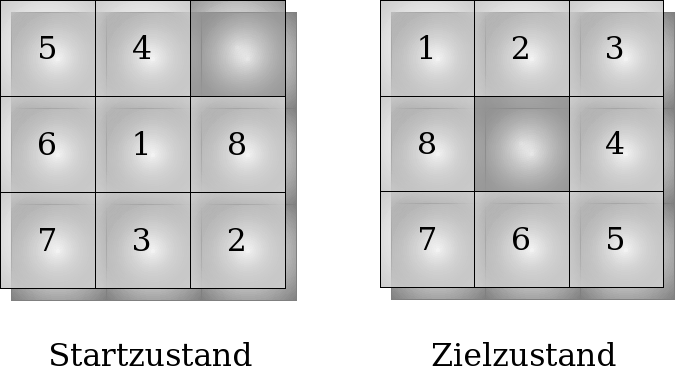
\includegraphics[scale=0.5]{8puz1.png}
\caption{Beispiel zum \textsc{8-puzzle} Problem}
\end{figure}

Beim \textsc{8-puzzle} Problem ist das Ziel, die Teile so zu bewegen, dass man vom Startzustand ausgehend den Zielzustand erreicht.
Die Beschr"ankung ist hierbei, dass man immer nur 1 Teil bewegen darf und sich niemals 2 Teile auf einem Feld befinden d"urfen.

Da sich in jedem Schritt 2 (freies Feld in der Ecke), 3 (freies Feld am Rand) oder 4 (freies Feld in der Mitte) Teile bewegen d"urfen, w"urde eine komplette Suche aller M"oglichkeiten mit Zugtiefe 20 zu 3.5*\(10^{9}\) oder, ignoriert man sich wiederholende Situationen, zu 9! Zust"ande f"uhren. ~\cite{Norv03}

Wie stellen wir nun fest, ob wir uns beim Bewegen eines Teiles auf die optimale L"osung zu bewegen oder uns entfernen?
Beim Ursprungsproblem k"onnen wir nur feststellen, ob ein Zustand dem Zielzustand entspricht oder nicht.
Wir m"ussen also ein vereinfachtes, sogenanntes \textsc{relaxed problem} finden, so dass Ueberschreitungen von Beschr"ankungen nicht zu einem Ignorieren des L"osungsschritt bzw. der L"osung f"uhrt.

Zuerst listen wir die Beschr"ankungen noch einmal getrennt auf:

Ein Teil darf
\begin{enumerate}
\item pro Schritt nur 1 Feld und 
\item nicht schr"ag und 
\item nur in ein freies Feld
\end{enumerate}
verschoben werden

Heben wir in diesem Fall die Beschr"ankung 3 einfach auf, d"urfen sich also Teile auch auf besetze Felder bewegen, wissen wir, dass die Summe der Schritte der Teile von ihren aktuellen Positionen zu den Zielpositionen die minimale Zahl der Schritte ist, die wir zur optimalen L"osung ben"otigen.
In diesem speziellen Fall wird das Manhattan distance genannt ~\cite{Norv03}
%[4, Seite 102]
Hebt man zus"atzlich noch Beschr"ankung 1 auf, erh"alt man eine Heuristik, die die Zahl der Teile die sich an falscher Position befinden beschreibt.

Nach ~\cite{Norv03} ist die erste Heuristik der zweiten Heuristik mit weniger Beschr"ankungen "uberlegen, f"uhrt also zu einer Suche mit geringerer durchschnittlichen Suchdauer.

Pr"uft man alle Kombinationen von Beschr"ankungsaufhebungen erreicht man so eine f"ur das jeweilige Problem optimale L"osung. Diesen Weg beschreitet \textsc{Absolver}. ~\cite{Norv03}
\\

\begin{figure}
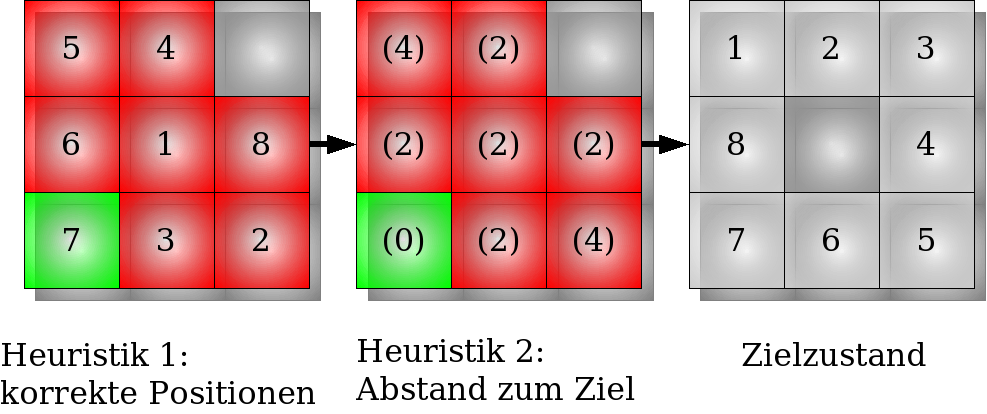
\includegraphics[scale=0.5]{8puz2.png}
\caption{2 m"ogliche Heuristiken zur L"osung von \textsc{8-puzzle}}
\end{figure}
                                                                                                                                                            
% text?

%~~ TODO: Ausf"uhrung
%~~ gibt noch andere m"oglichkeiten Heuristiken zu finden... 
%
\subsection{Formale Betrachtung des Problems}

Hat man nun eine heuristische Funktion gefunden kann man diese nun in einer Suche verwenden.

Das Grundger"ust der informellen Suche sieht erst einmal so aus:
\begin{samepage}
\textbf{\texttt{\begin{tabbing}\quad\quad\=\quad\kill
\textsc{Heuristische Suche}(Zustand alterZustand)\\
\emph{Solange} erstelleNeuenZustand(alterZustand,Bewertung()) \(\neq\) NULL\\
\>Zustand neuerZustand = erstelleNeuenZustand(alterZustand,Bewertung())\\
\emph{liefere als Ergebnis}(alterZustand)
\end{tabbing}}}
\end{samepage}

\emph{Zustand} ist je nach Problemdarstellung unterschiedlich, im Weiteren wird hier nur auf Graphendarstellungen eingegangen, da sich die meisten Probleme problemlos auf einen Graphen transformieren lassen k"onnen. Je nach Algorithmus werden hier auch pro Knoten unterschiedlich viele Daten gespeichert.

\emph{Bewertung} stellt unsere Heuristikfunktion h dar. Sie ist meistens vom Datentyp INTEGER, kann aber jede beliebige total geordnete Menge sein. Je nach Algorithmus mu"s sie speziellen Anforderungen gen"ugen.

\emph{erstelleNeuenZustand} entspricht unserer Funktion i, sie akzeptiert zum einen den momentanen Bearbeitungszustand und zum anderen die Heuristikfunktion \emph{Bewertung}.
Auf einige Beispiele f"ur m"ogliche h und i Funktionen wird nun in den n"achsten beiden Abschnitten n"aher eingegangen.
\nextpage
\section{Algorithmen 1. Gruppe - Schrittweiser Aufbau}
%~~best first search ueberhaupt erwaehnen? evtl 1. Gruppe in "best-first search" umbenennen
\subsection{Greedy Search}

Bei dem sogenannten \textsc{Greedy Search} w"ahlt die Funktion i den L"osungsschritt, von dem in der Funktion "ubergebenen Zustand \emph{alterZustand}, bei dem der Startknoten ge"offnet ist, m"oglichen L"osungsschritten, die den geringsten Wert f"ur h ausweisen. Es werden also nacheinander Knoten ge"offnet und die Bewertung aller S"ohne des jeweiligen Knotens miteinander verglichen. Der Knoten mit geringster Bewertung wird ausgew"ahlt und ge"offnet usw.
\begin{samepage}
\textbf{\texttt{\begin{tabbing}\quad\quad\=\quad\kill
\textsc{Greedy Search}(Zustand alterZustand)\\
\emph{Solange} erstelleNeuenZustand(alterZustand,Bewertung()) \(\neq\) NULL\\
\>Zustand neuerZustand = erstelleNeuenZustand(alterZustand,Bewertung())\\
\emph{liefere als Ergebnis}(alterZustand)\\
\\
Zustand erstelleNeuenZustand(Zustand momentanerZustand,Bewertung())\\
Knoten n = min(Bewertungsfunktion(ge"offnete Knoten von momentanerZustand))\\
momentanerZustand = SchliesseAlleKnoten(momentanerZustand) \\
%~~
\emph{Falls} "offneKnoten(momentanerZustand,n) \(\neq\) momentanerZustand\\
\>\emph{liefere als Ergebnis}("offneKnoten(momentanerZustand,n))
\end{tabbing}}}
\end{samepage}
%~~Kommentare
%~~Speicherverbrauch??
%~~~~ Problem: am besten das mit dem Ged"achtnis rausnehmen... weil das kommt ja bei A* eh...

Will man nun mit \textsc{Greedy Search} z.B. den k"urzesten Pfad in einem Graphen finden, bietet sich f"ur h die einfache Distanz "uber die Luftlinie an.

Also z.B. hier:\\
\begin{figure}[h]
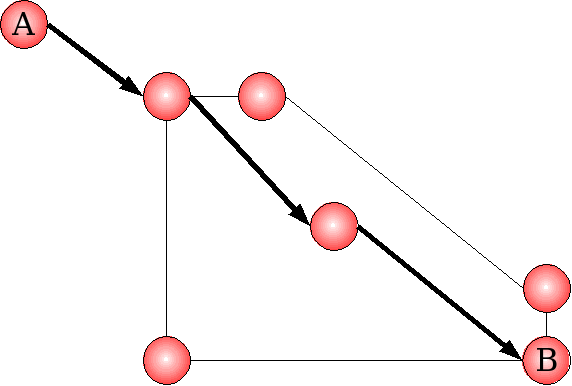
\includegraphics[scale=0.6]{gs1.png}
\caption{\textsc{Greedy Search} in Aktion}
\end{figure}

Leider hat der Algorithmus ein paar Nachteile:

\begin{figure}[h]
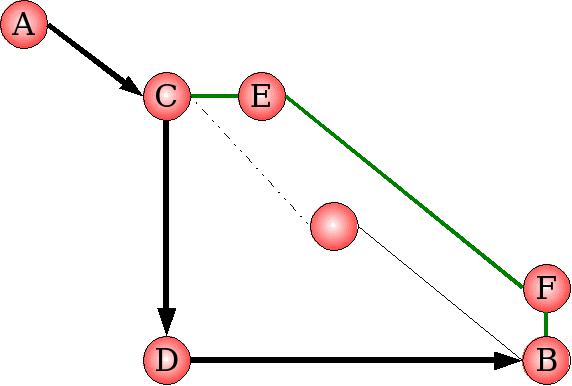
\includegraphics[scale=0.6]{gs2.png}
\caption{\textsc{Greedy Search} ist anf"allig gegen"uber falschen Starts}
\end{figure}

\begin{figure}[h]
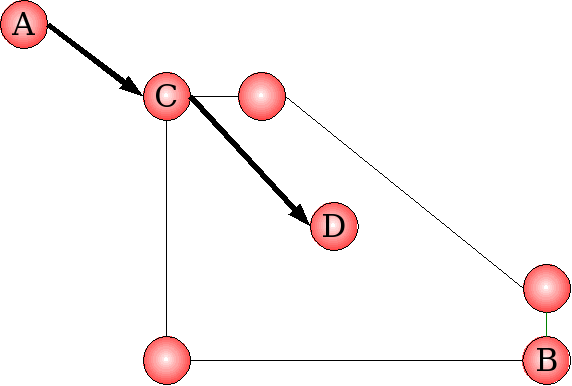
\includegraphics[scale=0.6]{gs3.png}
\caption{\textsc{Greedy Search} ist anf"allig gegen"uber Sackgassen}
\end{figure}

\begin{figure}[h]
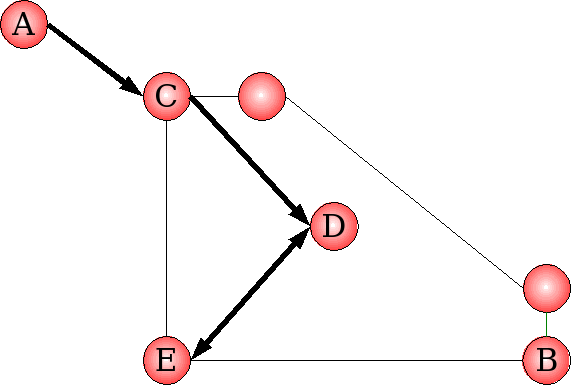
\includegraphics[scale=0.6]{gs4.png}
\caption{\textsc{Greedy Search} ist anf"allig gegen"uber Schleifen}
\end{figure}
Der \textsc{Greedy Search} Algorithmus ist weder optimal noch vollstaendig, f"uhrt jedoch in einigen F"allen zu einem relativ guten und schnellen Ergebnis.
In der Grundform hat der \textsc{Greedy search} Algorithmus einen Speicheraufwand von O(m), da nur der Weg zum Ziel und alle S"ohne des aktuell ge"offneten Knotens betrachtet werden. Pr"uft man auf Sackgassen und Schleifen, steigt der Speicheraufwand von O(b+m) auf O(\(b^{m}\)), wird aber trotzdem nicht optimal, wie in Abbildung 1.4 gezeigt und auch nicht vollst"andig, da er bei Graphen mit unendlich langen Pfaden nie terminiert. Mit Ged"achtnis hat er einen Zeitaufwand im schlechtesten Fall von O(\(b^{m}\)), da immer wieder r"uckgesprungen wird bis zwangsl"aufig alle Knoten (in einem endlichen Graphen) untersucht wurden.


\subsection{\textsc{Greedy Search} mit \textsc{CSPs}}

Hier nun ein weiteres Beispiel zu \textsc{Greedy Search} in Verbindung mit dem \textsc{Constraint Satisfaction Problem}, eine Landkarte so zu f"arben, dass kein Land die gleiche Farbe wie ein angrenzendes Land besitzt und dabei eine bestimmte Zahl von unterschiedlichen Farben nicht "uberschreitet. Als Heuristik bietet sich \textsc{Most-Constrained Variable} ~\cite{Norv03} an, wir beginnen also mit der F"arbung eines Landes und nehmen als n"achstes Land jenes, welches ungef"arbt ist und die meisten gef"arbten Nachbarn besitzt. Welche Farbe wir dann w"ahlen ist beliebig, solange sie nicht mit einer angrenzenden Farbe in Konflikt ger"at. Wie man an diesem Beispiel sieht, arbeitet die heuristik zusammen mit \textsc{Greedy Search} sehr erfolgreich. Als Basis f"ur dieses Beispiel diente die Europakarte von ~\cite{Worldmap}

\begin{figure}[h]
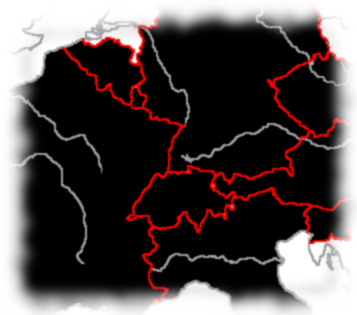
\includegraphics[scale=0.7]{e11.png}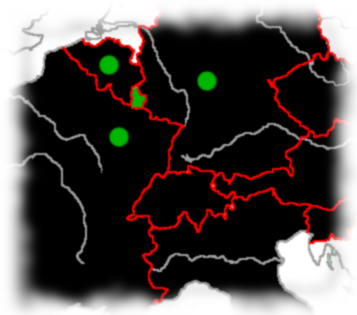
\includegraphics[scale=0.7]{e12.png}\\
\caption{Der Algorithmus \textsc{Greedy Search} mit Heuristik der \textsc{Most-constrained Variable} beginnt zuf"allig in Lichtenstein}
\end{figure}[h]

\begin{figure}[h]
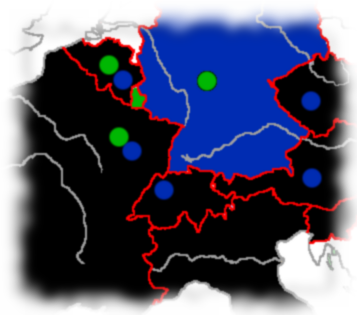
\includegraphics[scale=0.7]{e13.png}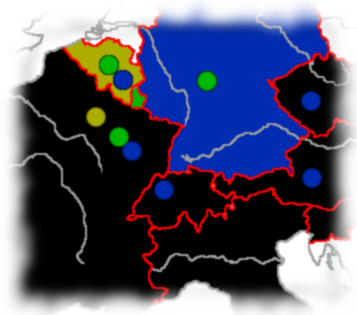
\includegraphics[scale=0.7]{e14.png}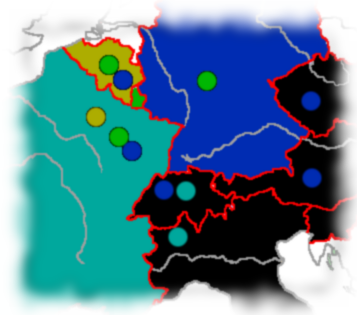
\includegraphics[scale=0.7]{e15.png}\\
\caption{Deutschland und Belgien wird gew"ahlt, dann Frankreich wegen 3 Punkten}
\end{figure}[h]

\begin{figure}[h]
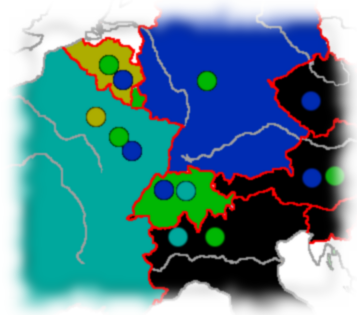
\includegraphics[scale=0.7]{e16.png}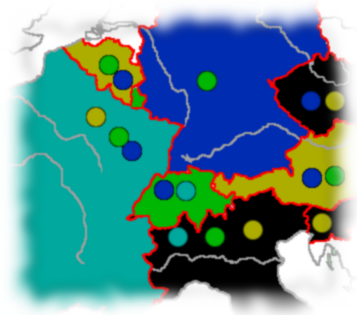
\includegraphics[scale=0.7]{e17.png}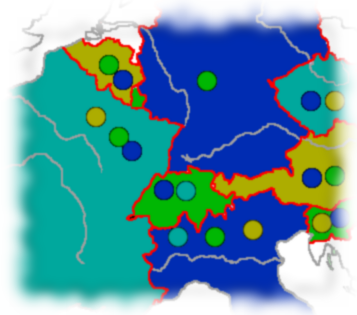
\includegraphics[scale=0.7]{e18.png}\\
\caption{"Die Schweiz und dann "Osterreich werden mit 2 Punkten, Italien danach mit 3 Punkten gew"ahlt, der Rest wird aufgef"ullt}
\end{figure}[h]

\nextpage

\subsection{Verbesserungen von \textsc{Greedy Search: A*}}

Erweitert man die Funktion i, dass nicht nur die Kinder des gerade ge"offneten sondern aller der noch nicht besuchten Knoten betrachtet erhalten wir einen vollst"andigen Algorithmus.
Dadurch treten nun keine Schleifen und Sackgassen mehr auf, es wird einfach an die n"achste passende Stelle gesprungen.
%~~~ Ged"achtnis rausnehmen also naja...
\begin{samepage}
\textbf{\texttt{\begin{tabbing}\quad\quad\=\quad\kill
\textsc{A* Search}(Zustand alterZustand)\\
\emph{Solange} erstelleNeuenZustand(alterZustand,Bewertung()) \(\neq\) NULL\\
\>Zustand neuerZustand = erstelleNeuenZustand(alterZustand,Bewertung())\\
\emph{liefere als Ergebnis}(alterZustand)\\
\\
Zustand erstelleNeuenZustand(Zustand momentanerZustand,Bewertung())\\
Knoten n = min(Bewertungsfunktion(ge"offnete Knoten von momentaner Zustand))\\
\emph{Falls} "offneKnoten(momentanerZustand,n) ungleich momentanerZustand\\
\>\emph{liefere als Ergebnis}("offneKnoten(momentanerZustand,n))
\end{tabbing}}}
\end{samepage}

\begin{figure}[h]
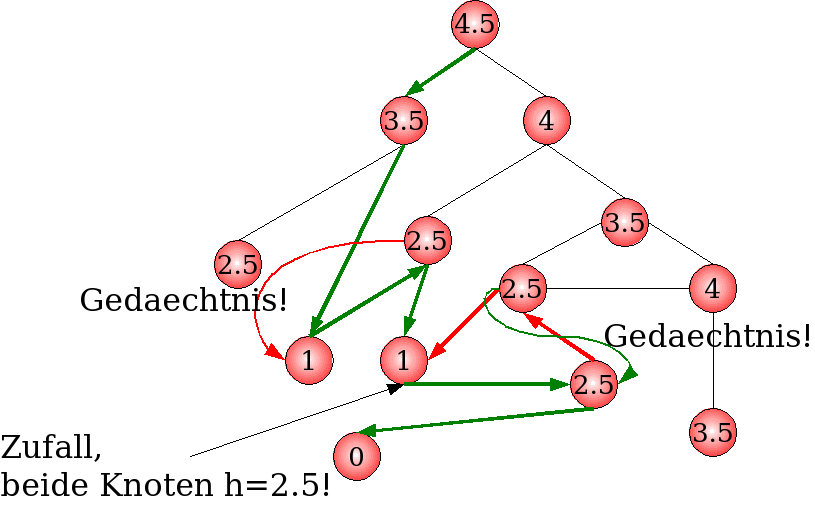
\includegraphics[scale=0.6]{a1.png}
\caption{\textsc{Greedy Search} mit Ged"achtnis}
\end{figure}

Leider ist dieser Algorithmus immer noch anf"allig gegen"uber einem ung"unstigen Start und in vielen F"allen nicht optimal.
Deshalb hat man den sogenannten A* Algorithmus entwickelt, der die gleiche i Funktion aufweist, dessen Bewertungsfunktion h aber eine Kombination aus den bereits bekannten \textsc{Greedy Searchs} und \textsc{Uniform-cost Searchs} ist.

Hier ist also\\
\textbf{(n) = (Enternung von n zum Ziel (Luftlinie) + Kantenl"ange von Start bis n)}

\emph{Bemerkung:}\\
Man kann h auch beliebig anders w"ahlen, A* bleibt aber nur solange optimal wie die Heuristik h der Dreiecksgleichung gen"ugt, d.h. zu einer gegebenen Heuristik h und einer direkten Verbindung zweier Punkte A und B darf es keine andere Verbindung zwischen A und B mit einem Knoten C geben, bei der h(B "uber C) \textless h(B "uber A) gilt. Eine genauere Beschreibung und eine M"oglichkeit derartige heuristische Funktionen zu korrigieren findet man in der Literatur ~\cite{Norv03}.

\begin{figure}[h]
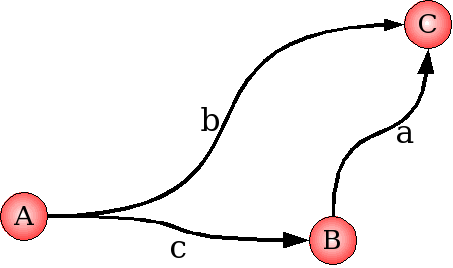
\includegraphics[scale=0.6]{3eck.png}
\caption{Dreiecksungleichung und A*: A* ist optimal wenn h(b) \textless h(a) + h(c) f"ur alle a,b,c, wobei c die k"urzeste Verbindung von A nach C darstellt.}
\end{figure}

Ein Beispiel das zeigt, dass z.B. ,,Luftlinie`` nicht immer die k"urzeste Verbindung darstellt, w"are das sogenannte \textsc{Brachistochrone} Problem, also die Frage nach dem \emph{schnellsten} Weg von A nach B:

\begin{figure}[h]
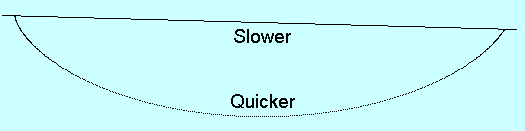
\includegraphics[scale=0.6]{Cycloid2Slope.png}
\caption{\textsc{Brachistochrone} Problem - Was ist der \emph{schnellste} Weg von links nach rechts? ~\cite{evo}}
\end{figure}

Untersuchungen erbrachten die Ergebnisse, dass A* optimal und vollst"andig ist und auch, dass es keinen anderen optimalen und vollst"andigen Algorithmus gibt, der (f"ur eine beliebige heuristische Funktion) die Aufgabe mit Expandierung von weniger Knoten schafft. ~\cite{Norv03}

Im Folgenden wird nun anhand des bekannten Beispiels die Funktionsweise von dem \textsc{A* Search} Algorithmus demonstriert. Zahlen in den roten Knoten bedeuten wie vorher auch die Distanz mittels Luftlinie, in den gr"unen Knoten der Wert der heuristischen Funktion, bisherige Kantenl"ange + Distanz Luftlinie. Ein * markiert einen Knoten, f"ur den ein besserer Weg gefunden wurde.
\\
\begin{figure}[h]
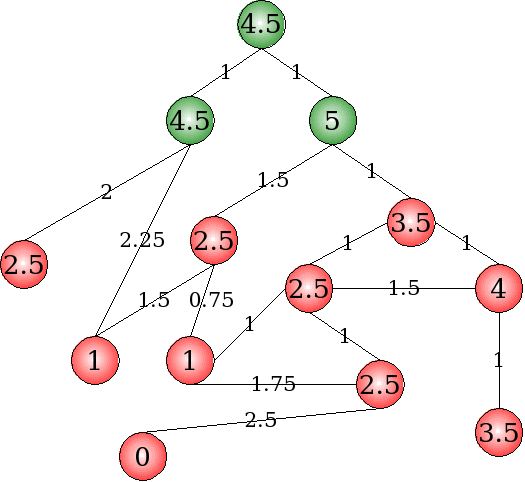
\includegraphics[scale=0.6]{a4.png}
\caption{\textsc{A* Search}, Startzustand}
\end{figure}
\begin{figure}[h]
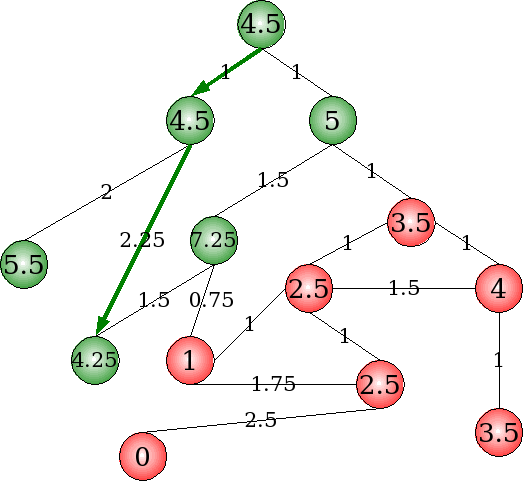
\includegraphics[scale=0.6]{a5.png}
\caption{\textsc{A* Search}, erster und zweiter Schritt}
\end{figure}
\begin{figure}[h]
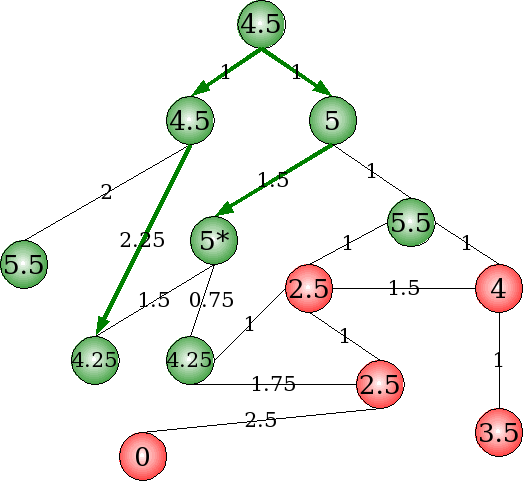
\includegraphics[scale=0.6]{a6.png}
\caption{\textsc{A* Search}, dritter und vierter Schritt}
\end{figure}
\begin{figure}[h]
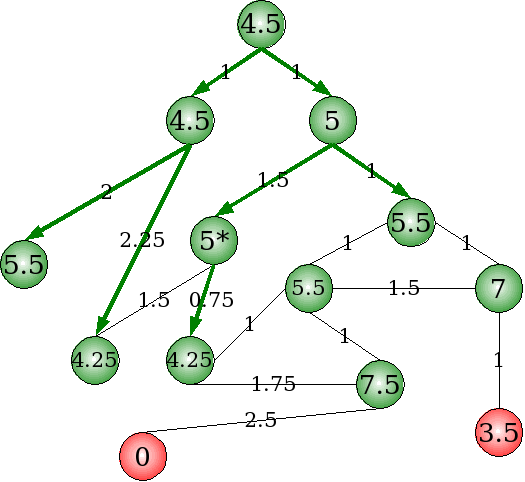
\includegraphics[scale=0.6]{a7.png}
\caption{\textsc{A* Search}, restliche Schritte}
\end{figure}
\begin{figure}[h]
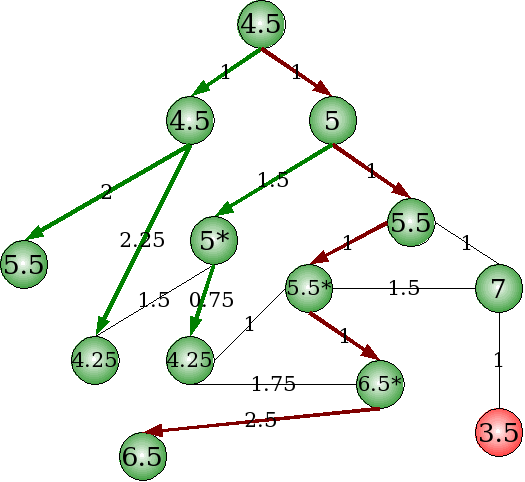
\includegraphics[scale=0.6]{a8.png}
\caption{\textsc{A* Search}, Endzustand: optimaler Weg gefunden}
\end{figure}

A* hat in seiner Grundform ebenfalls einen Zeit und Speicheraufwand von O(\(b^{m}\)), da wie beim uniform cost search alle ge"offneten Knoten im Speicher liegen und im schlechtesten Fall auch alle Knoten untersucht werden m"ussen. 
F"ur b = 2 und m = 40 ben"otigt ein Aldi-Rechner f"ur A* im schlechtesten Fall vielleicht eine Stunde. Der Speicherbedarf dagegen ist im schlechtesten Fall dagegen mit 1024 GB jenseits von gut und b"ose.
Der Speicheraufwand l"asst sich jedoch mit einem etwas abgewandelten Algorithmus reduzieren. Zum Gl"uck gibt es mehrere verschiedene derartige Algorithmen, im Folgenden werden zwei vorgestellt.

\subsection{\textsc{Iterative Deepening A* Search}}

\textsc{IDA* Search} funktioniert im Grunde wie der bereits betrachtete \textsc{Iterative Deepening Search}, statt Knotentiefe als Grenze wird hier aber ein Kostenlimit gesetzt. Es werden also immer nur ein Bereich aus Knoten untersucht, deren Bewertungsfunktion h kleiner als das Kostenlimit ist. Das Speicherersparnis kommt nat"urlich um den Preis der Geschwindigkeit. Zwar werden pro Schritt weniger neue Knoten betrachtet, daf"ur m"ussen alle noch nicht besuchten Knoten in Suchtiefenreichweite neu berechnet werden. Dass dies keinen so gro"sen Einflu"s auf die Laufzeit hat, ergibt sich wie beim \textsc{Iterative Deepening Search} aus der Tatsache, dass in den mei"sten F"allen die unterste Ebene des Graphen die meisten Knoten enth"alt.

Die Qualit"at des \textsc{Iterative Deepening A* Search} ergibt sich aus der Zahl der unterschiedlichen Werte die die Heuristikfunktion annehmen kann, da pro Schritt die Suchtiefe auf den n"achstgr"o"seren Wert geschaltet wird. Eine Suche in Graphen mit reellwertiger Heuristikfunktion kann also zu einem unendlich langen Unterfangen werden, der Algorithmus ist also weder vollst"andig, noch optimal, wie folgendes Beispiel nochmals verdeutlicht:

%~~ TODO Beispiel

\subsection{\textsc{Simplified Memory-Bounded A* Search}}

\textsc{SMA* Search} verbraucht keine feste Speichermengenge, sondern passt sich an den verf"ugbaren Speicherplatz an, versucht also so viele Knoten wie m"oglich zu speichern. Der Algorithmus beginnt, falls der Speicherplatz knapp wird, bereits berechnete Teile des Graphen durch das jeweilige Minimum der Heuristikfunktionen aller enthaltenen Knoten zu ersetzen. Ist letzteres nie der Fall, arbeitet der Algorithmus also genau wie \textsc{A* Search} und ist vollst"andig, sofern genug Speicherplatz f"ur die L"osung mit Suchtiefe m, also O(b*m) zur Verf"ugung steht. Er ist auch optimal nach ~\cite{Norv03}.

\nextpage
\section{Algorithmen der 2. Gruppe - Schrittweise Verbesserung}

Optimal und vollst"andige Algorithmen sind sch"on und gut, in der Praxis sind die Probleme jedoch meist zu komplex oder es liegen sowieso keine gesicherten Werte vor, so dass es oft schon reicht, wenn nicht die optimale L"osung sondern nur z.B. eine 5\% am Optimum liegende L"osung gefunden werden kann.
Diese Aufgabe k"onnen die Algorithmen der zweiten Gruppe sehr erfolgreich l"osen. Wie anfangs erw"ahnt werden bei diesen Algorithmen die L"osung nicht Schritt f"ur Schritt aufgebaut sondern fertige L"osungen generiert und diese iterativ verbessert.
Wichtig ist dabei, dass die Aufgabenstellung so umgeschrieben wird, dass jede Art von Ergebnis g"ultig ist, also einer bestimmten Qualit"atsstufe, der sogenannten Fitness, zugeordnet werden kann.
Dazu werden harte Nebenbedingungen, also z.B. Lager"uberschreitungen, Bargeld"uberschreitungen, Zeit"uberschreitungen etc. mit Strafkosten belegt, also die Fitness gesenkt, anstatt dass die L"osung ganz verworfen wird.
Der grosse Unterschied zur ersten Gruppe ist aber, dass die neuen L"osungen mehr oder weniger zuf"allig generiert werden. Dadurch ergibt sich das Problem, dass man nie genau weiss, ob bei weiteren Durchl"aufen bessere L"osungen gewonnen werden k"onnen oder nicht.

Grunds"atzlich arbeiten Algorithmen der 2. Gruppe wie folgt:
%~~ englisch/deutscher Name
\begin{samepage}
\textbf{\texttt{\begin{tabbing}\quad\quad\=\quad\quad\=\kill
Schrittweise Verbesserung()\\
Losung alteL"osung = erstelleZuf"alligeL"osung()\\
\emph{Wiederhole}\\
\>L"osung neueL"osung = i(alteL"osung)\\
\>\(\triangle\)= h(neueL"osung) - h(alteL"osung)\\
\>\emph{Falls} selektion( T, \(\triangle\) ) == true\\
\>\>\emph{Dann} alteL"osung = neueL"osung\\
\emph{bis} alteL"osung ausreichend gut\\
\emph{liefere als Ergebnis}(alteL"osung)
\end{tabbing}}}
\end{samepage}
%~~datentyp von Differenz?
%~~Selektion != i ??

Hier sind 2 neue Funktionen hinzugekommen, die jedoch nicht weiter kompliziert sind.
\emph{erstelleZuf"alligeL"osung} erstellt wie der Name schon sagt, eine zuf"allige Startl"osung, die dann schrittweise verbessert werden soll.
\emph{selektion} pr"uft in Abh"angigkeit einer Variablen T, ob \(\triangle\) ausreichend klein ist.\\
Auf einige Beispiele f"ur h, i und selektion m"ochte ich hier eingehen:

\subsection{\textsc{Hill-Climbing Algorithmus}}

Der einfachste darauf basierende Algorithmus ist der sogenannte \textsc{Hill-Climbing} Algorithmus. Der Name r"uhrt von dem anschaulichen Problembeispiel her, dass man sich alleine im Gebirge befindet, im Nebel nichts sehen kann, aufgrund Sauerstoffknappheit sich nicht an seine letzten Schritte erinnern kann und als Ziel hat, den h"ochsten Berggipfel zu erreichen. Eine m"ogliche Strategie w"are, dass man sich vortastet, ob man denn mit dem n"achsten Schritt etwas h"oher kommt oder nicht.\\

Hier in diesem Beispiel m"ochten Bergsteiger B, C und D zum h"ochsten Punkt A.

\begin{figure}[h]
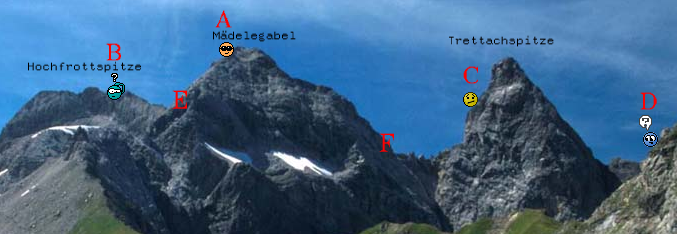
\includegraphics[scale=0.6]{berg.png}
\caption{3 Bergsteiger auf der Suche nach dem Gipfel, Grundlage f"ur Bild von  ~\cite{Berg}}
\end{figure} 

Beim Hill-Climber ist T = 0 und die \textsc{Selection} Funktion sieht so aus:
\begin{samepage}
\textbf{\texttt{\begin{tabbing}\quad\quad\=\quad\kill
Selection(T, \(\triangle\))\\
\emph{Falls} \(\triangle\) \textless T\\
\>\emph{liefere als Ergebnis}(true)\\
\emph{liefere als Ergebnis}(false)
\end{tabbing}}}
\end{samepage}

Es werden also schlechtere L"osungen sofort verworfen, alle anderen weiterverwendet.

\subsection{Probleme des Hill-Climbing Algorithmus}

Bei dem Algorithmus ergeben sich aber zwei schwerwiegende Probleme:

\textbf{1. der Algorithmus wird mit hoher Wahrscheinlichkeit an einem lokalen Optimum h"angenbleiben}

Betrachtet man hier Bergsteiger C und D werden diese, folgen sie der Ansteigung der Trettachspitze, zwar ziemlich hoch hinaus kommen, werden A jedoch nicht erreichen sondern im lokalen Optimum der Trettachspitze stecken bleiben. Zwar m"usste C einfach nach links laufen um A zu erreichen, da er aber nicht weiss, dass A links von ihm liegt, ist er nicht besser dran als D.

Dies l"asst sich beheben, indem man den Algorithmus nach einiger Zeit ohne Verbesserung einfach mit einer anderen Startkonfiguration/position neu beginnt, die beste Fitness der bisherigen Durchl"aufe aber speichert. Dann nennt man es einen \textsc{Random-Restart Hillclimbing} Algorithmus. In diesem Fall m"usste C irgendwo zwischen E und F neustarten um auf direktem Wege zu A zu kommen.
Problem bleibt hier festzustellen, ob wir denn in einem lokalen Optimum oder einer Kante stecken oder nicht schon kurz vor dem Ziel sind.

\textbf{2. die Fitnesslandschaft ist oft sehr ,,wild`` also mit grossen Gradientenunterschieden besetzt}

Hier hilft auch kein zuf"alliges Neustarten mehr, man wird wahrscheinlich fast alle L"osungsm"oglichkeiten durchsuchen m"ussen, der Algorithmus ist also wieder nicht viel besser als eine einfache zuf"allige Suche "uber dem L"osungsraum. Leider sind die meisten praktischen Probleme von dieser Art, somit liegt die Hauptschwierigkeit beim Hillclimber also nicht bei der Suche selbst sondern bei der Gestaltung der Problemstellung, so dass eine Fitnesslandschaft mit m"oglichst sanften Steigungen entsteht.

\textbf{3. in der Fitnesslandschaft gibt es Plateaus}

Auf Plateaus, also Gebieten mit gleichem Fitnesswert reduziert sich die Effektivit"at des \textsc{Hill-Climbers} auf die eines \textsc{Random-Walks} also einer rein zuf"alligen Suche, es gibt keinen Anhaltspunkt, ob eine Position der anderen "uberlegen ist.
Mit Plateaus kann man im Algorithmus nur schwer umgehen, die beste L"osung ist, die Fitnesslandschaft z.B. durch Einf"uhrung zus"atzlicher Faktoren die in die Bewertungsfunktion eingehen die Fitnesslandschaft selbst zu ver"andern. In diesem Fall ist B ziemlich ratlos, aber vielleicht weiss er ja, dass an der linken Seite der M"adelegabel ein leichtes L"uftlein pfeift wonach er sich orientieren k"onnte\dots 

\subsection{Simulated Annealing Algorithmus}

"Ahnlich funktioniert auch das sogenannte \textsc{Simulated Annealing}, das urspr"unglich aus der Physik kommt.
Wird eine bessere L"osung gefunden, wird sie wie beim Hillclimber auf jeden Fall weiterverwendet, wird eine schlechtere L"osung gefunden, wird sie nicht sofort verworfen, sondern mit einer Wahrscheinlichkeit die der Parameter T angibt weiterverwendet.
Ueber die Generationen wird T dabei immer weiter verringert, bis f"ur T = 0 (hoffentlich) eine ziemlich gute L"osung gefunden wurde.
Es werden f"ur grosse T also praktisch alle L"osungen weiterverwendet, bis auf die, die deutlich schlechter sind.

\begin{figure}
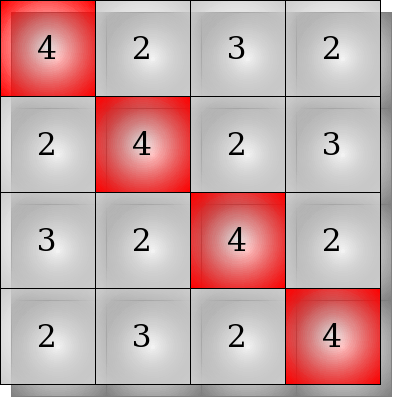
\includegraphics[scale=0.6]{dame1.png}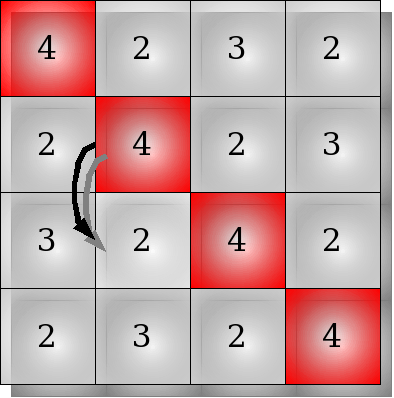
\includegraphics[scale=0.6]{dame2.png}
\caption{Packungsproblem als Beispiel f"ur ,,Simulated Annealing``}
\end{figure}

Es gibt viele weitere Variationen von Selektion und T, auf die hier im speziellen nicht eingegangen wird, aber im Ausblick am Schluss noch einmal erw"ahnt werden.~~

\subsection{Heuristik des minimalen Konflikts bei CSPs}

Heuristische Algorithmen der 2. Gruppe eignen sich sehr gut um \textsc{CSP} Probleme wie z.B. das n-Damenproblem zu l"osen. Mit der nun beschriebenen Heuristik kann z.B. das Millionen-Damen Problem im Durschnitt mit weniger als 50 Schritten gel"ost werden. ~\cite{Norv03}

Wieder ist der Trick, nicht perfekte L"osungen zu suchen, sondern eine zuf"allige zu generieren diese Schritt f"ur Schritt zu ,,reparieren`` (sogenanntes ,,heuristic repair`` ~cite{Norv03}).
Das Optimierungsproblem zu n-Dameproblem lautet ,,Finde eine Position in der m"oglichst wenige Damen von m"oglichst wenigen anderen Damen geschlagen werden k"onnen``.

Hier nun zur Uebersicht ein Beispiel zum 4 Dameproblem in 5 Schritten:

W"ahrend die roten Felder die Positionen der 4 Damen darstellen, geben die Zahlen den Wert der Heuristik an.
Die Heuristik ist eine sogenannte ,,min conflicts``[6] Heuristik, die jeweils angibt, wieviele Bedingungen bei einer Konfiguration "uberschritten wird.
In diesem Fall entspricht dies der Zahl der Damen, die das Feld angreifen, bei roten Feldern inklusive dieser Dame selbst.
Bei jedem Reperaturschritt der ung"ultigen L"osung wird nun f"ur eine Dame einer zuf"alligen Spalte ein zuf"allig Feld mit niedrigerer oder gleicher Bewertung gew"ahlt.

%Programm evtl?

\begin{figure}[h]
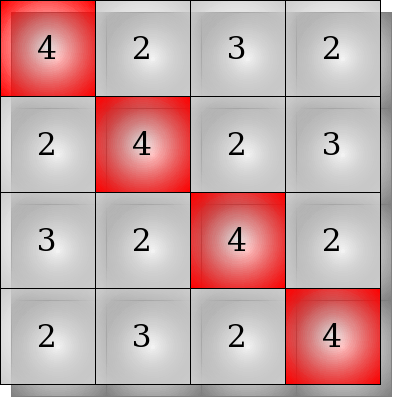
\includegraphics[scale=0.6]{dame1.png}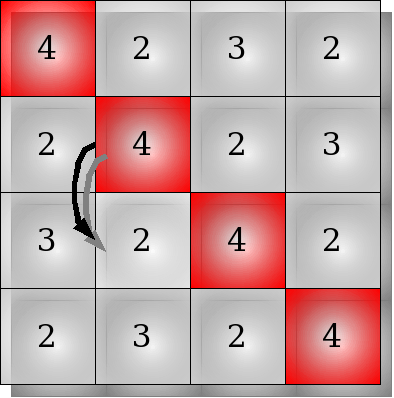
\includegraphics[scale=0.6]{dame2.png}
\caption{\textsc{CSP} mittels Heuristik des minimalen Konflikts}
\end{figure}
                                                                                                                                                            
In diesem Beispiel stehen alle 4 Damen in einer Diagonalen, also k"onnen z.B. in der Diagonalen 4 Damen jeweils ein Feld angreifen bzw. stehen darauf. 
Hier wurde die 2. Spalte gew"ahlt und die Dame auf das niedriegere Feld in der 3. Zeile verschoben.
Dass diese Heuristik scheinbar funktioniert, kann man auch daran erkennen, dass die Gesamtzahl der angegriffenen Damen sich von 16 nun auf 8 verringert hat:

\begin{figure}[h]
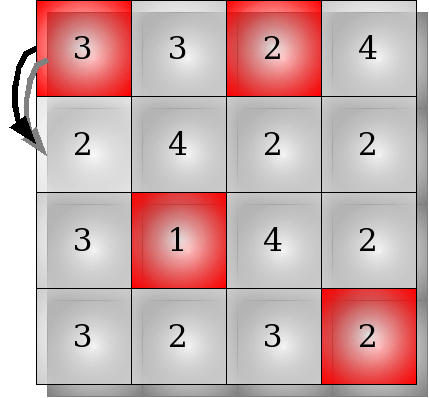
\includegraphics[scale=0.6]{dame3.png}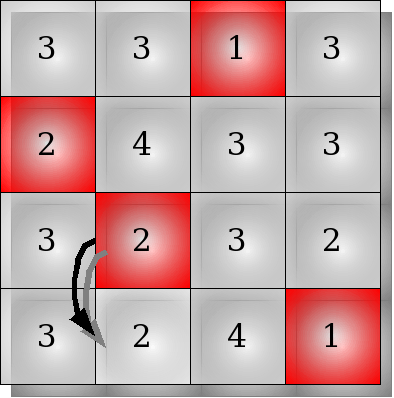
\includegraphics[scale=0.6]{dame4.png}
\caption{\textsc{CSP} mittels Heuristik des minimalen Konflikts}
\end{figure}

Im ersten Bild ist hier die Wahl der ersten Spalte zwingend, mit keiner anderen Dame findet man ein besseres Feld.
In der Situation im zweiten Bild w"urde der \textsc{Hill-Climber} sich auf einem Plateau befinden und w"are nicht besser wie eine zuf"allige Suche. 

\begin{figure}[h]
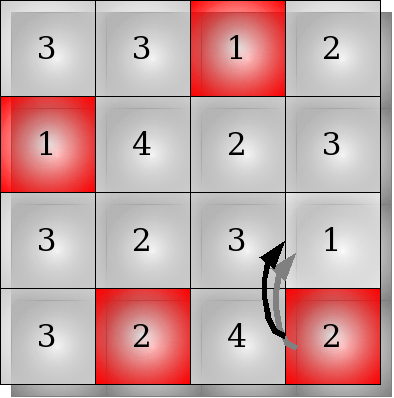
\includegraphics[scale=0.6]{dame5.png}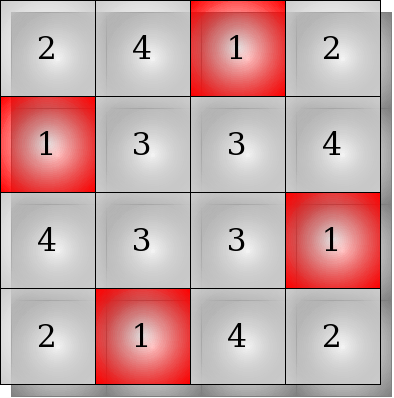
\includegraphics[scale=0.6]{dame6.png}
\caption{\textsc{CSP} mittels Heuristik des minimalen Konflikts}
\end{figure}

Im letzten Bild gibt es keine Verbesserung und der \textsc{Hill-Climber} l"auft ohne Verbesserung bis zum Abbruch ohne Ver"anderung weiter. Da wir aber das Optimum, d.h. es gibt eine L"osung f"ur das n-Damenproblem mit keiner Ueberschneidung, schon kennen und es hier auch abz"ahlen k"onnen, sind wir fertig.

\subsection{Verbesserte Hill-Climbing Algorithmen}

Es gibt einige Verfeinerungen des \textsc{Hill-climbing} Algorithmus, besonders erw"ahnenswert sind die \textsc{evolution"aren Algorithmen}. Diese finden z.B. Anwendung in komplexen praktischen Problemstellungen wie z.B. Betriebsplanoptimierung an der SAP schon l"anger erfolgreich arbeitet.  ~\cite{SAP}
Grob gesagt, handelt es sich bei dabei um \textsc{Hill-climber}, der nicht jede L"osung verwirft, zusammen mit einer Breitensuche in Form von einer Population von konkurrierenden L"osungen.

Die sogenannten \textsc{Genetic Algorithms} gehen noch einen Schritt weiter, trennen Ph"anotyp, also die endg"ultige L"osung, komplett vom Genotyp, der Datenstruktur, auf die die Mutationsoperatoren angewendet werden. Ausserdem f"ugen sie dem ganzen noch eine Art Ged"achtnis in Form von dominant/rezessiver Gene, inaktiver Gene, sogenannter Introne, die nicht tats"achlich in einem Ph"anotyp codiert werden, sondern nur als Mutationsschutz dienen, und mit einer Rekombination der Genstrukturen zweier L"osungen mittels \textsc{Crossing Over} hinzu.
Genauer kann darauf hier leider nicht eingegangen werden, da es den Rahmen dieses Dokuments sprengen w"urde. Sehr empfehlenswert ist hierzu das Buch "Genetic Programming - An Introdution". ~\cite{Banz98}
Auf jeden Fall sind in einigen Problemgebieten, verglichen mit anderen Suchstrategien, sehr erfolgreich, denn welch anderer Algorithmus kann schon Vortr"age "uber sich selbst halten?

\nextpage
\section{Zusammenfassung}

\subsection{Allgemeine Suchalgorithmen}
\textpage
\subsection{Heuristische Suchalgorithmen}

Insgesamt hat man im zweiten Teil gesehen, dass wir die Zahl der zu untersuchenden M"oglichkeiten durch Heuristiken stark reduzieren k"onnen. Zwar bieten die Heuristiken keine Garantie fur eine schnellere Ausfuhrung, die schlechteste Laufzeit betr"agt nach wie vor O(\(b^{m}\)), im praktischen Anwendungsfall mit einer guten Heuristik l"asst sich jedoch die durchschnittliche Suchzeit stark reduzieren.

Das Hauptproblem lag darin, dass eine passende heuristische Funktion je nach Problem zu finden. Das Ergebnis war, dass durch Benutzung von einfach zu bestimmenden Heuristiken des sogenannten \textbf{relaxed problem} die urspr"ungliche L"osung auch gut handhabbar wird. Diese wurden dann von dem \textsc{Greedy Search} Algorithmus verwendet, der zwar L"osungen in geringen Zeitaufwand finden konnte, indem er jeweils den besten Knoten w"ahlte und auf das Ziel marschierte, jedoch weder optimal noch vollst"andig war.

Indem die Idee des \textsc{Uniform Cost Search} Algorithmus, den bisherigen Weg in die heuristische Funktion einzubeziehen, egab sich der \textsc{A* Search}, der einen guten und vor allem optimalen und vollst"andigen Algorithmus darstellte. Probleme bereiteten jedoch der immense Speicherverbrauch, da beim \textsc{A* Search} im schlechtesten Fall alle Knoten im Speicher behalten werden m"ussen. 

Dagegen wurden gleich zwei M"oglichkeiten aufgezeigt, einerseits der \textsc{Iterative Deepening A* Search}, der auf Kosten der Vollst"andigkeit, Optimalit"at und Berechnungszeit den Speicherverbrauch stark reduzierte. Eine kl"ugere Herangehensweise hatte dagegen der \textsc{Simplified Memory-Bounded A* Search} an den Tag gelegt, in dem er einfach so viel wie verf"ugbar Speicherplatz verwendete und, wieder auf Kosten der Geschwindigkeit, Knoten die wahrscheinlich nicht Teil der L"osung waren verga"s. Es wurde gezeigt, dass der Algorithmus sogar optimal und vollst"andig ist, falls genug Speicher zur Verfugung steht.

Anschlie"send wendeten wir uns den Algorithmen zu, die die L"osung nicht schrittweise aufbauten sondern schrittweise ,,reparierten``. Das Problem wurde dabei als Optimierungsproblem umschrieben und es wurden fertige L"osungen meist durch Zufall generiert und deren Qualit"at bestimmt. Die meisten Algorithmen die darunter fallen sind nicht optimal oder vollst"andig, da sie auf Zufall basieren. 

Der \textsc{Hill-climbing} Algorithmus verwarf die schlechteren L"osungen einfach und ver"anderte die (scheinbar) guten L"osungen rekursiv weiter. Zwar konnte man durch den \textsc{Random restart Hill-climbing} gewisse lokale Optima vermeiden, die eigentliche Hauptarbeit zur Vermeidung lokaler Optima liegt jedoch nicht beim Gestalten des Suchalgorithmus sondern des L"osungsraums selbst. 

\textsc{Simulated Annealing} hat dazu den Ansatz gebracht, dass auch schlechtere L"osungen unter Umst"anden in die n"achste Generation weiterverwendet und weiter zuf"allig ver"andert wurden. Anschaulich entspricht dieser Algorithmus dem langsamen Abk"uhlen eines Stoffes bis dessen minimaler Energiezustand (das Optimum!) erreicht ist. 

Zum Schluss wurde ein Ausblick auf verbesserte Algorithmen dieser Art gemacht, die durch die nat"urliche Evolution in der Natur inspiriert wurden. Darunter fallen die sogenannten \textsc{Genetic Algorithms} die sich besonderer Techniken der Rekombination neuer L"osungen und des Ged"achtnisses an verworfene L"osungen bedienen und Anwendbarkeit auf komplexe, praktische Probleme bewiesen haben.

\begin{thebibliography}{99}
\bibitem{Norv03} {\sc Russel S., Norvig P.:}  \textit{Artificial Intelligence -- A Modern Approach}, 
Second Edition, Prentice Hall, 2003.
\bibitem{Worldmap} {\sc Brion L. Vibber:}  \textit{Maps of the World},
http://leuksman.com/misc/maps.php
\bibitem{Berg} {\sc D. Jonderko:}  \textit{bergfieber.de},
http://www.bergfieber.de/berge/frameset.htm
\bibitem{SAP} {\sc Dr. Heinrich Braun:}  \textit{Evolution�re Algorithmen im SAP Supply Chain Management},
http://www.aifb.uni-karlsruhe.de/AIK/aik\_07/AIK2001Braun.pdf
\bibitem{Banz98} {\sc Banzhaf W., Nordin P., Keller R., Francone F.:}  \textit{Genetic Programming - An Introduction},
Morgan Kaufmann Publishers, Inc. 1998

%evtl noch benutzte Software eintragen, openoffice, vim, gimp, texi2pdf
\end{thebibliography}
%TODO: Fett/Kursiv rein, Sonderzeichen etc.
\end{document}

